%
% A new installer for TeX Live
% Norbert Preining, Reinhard Kotucha, Siep Kroonenberg
% Article presented on the 16th BachoTeX meeting, Bachotek ?? May 2008
%
% Copyright 2007 Norbert Preining at al.
% You can redistribute and/or modify this document under the terms of the
% GNU General Public License as published by the Free Software Foundation;
% either version 2 of the License, or (at your option) any later version.
%
%\documentclass{arstexnica}
\documentclass{ltugproc}
\usepackage[latin1]{inputenc}
\usepackage[T1]{fontenc}
\usepackage{lmodern}
\usepackage[english]{babel}
\usepackage{graphicx}
\usepackage{fancyvrb}
\usepackage{url}
\usepackage{marvosym}
\usepackage{listings}
\lstset{frame=lines,basicstyle=\ttfamily,showspaces=true,prebreak={\Righttorque},postbreak={\Lefttorque},breaklines}
\usepackage{microtype}

\usepackage{hyperref} % should be loaded last because it patches other
                      % packages.

\newcommand{\tl}{\TeX~Live}
\newcommand{\ctan}{CTAN}
\newcommand{\tpm}{\texttt{tpm}}
\newcommand{\tpms}{\tpm{}s}
\newcommand{\tlpsrc}{\texttt{tlpsrc}}
\newcommand{\tlpsrcs}{\tlpsrc{}s}
\newcommand{\tlpobj}{\texttt{tlpobj}}
\newcommand{\tlpobjs}{\tlpobj{}s}
\newcommand{\tlpdb}{\texttt{tlpdb}}
\newcommand{\tlpdbs}{\tlpdb{}s}

\newcommand{\pl}{Perl}
\newcommand{\gs}{Ghostscript}
\newcommand{\tlu}{\texttt{texlua}}
\newcommand{\kpse}{\texttt{kpathsea}}

% from l2tabuen:
\tolerance 1414
\hbadness 1414
\emergencystretch 1.5em
\hfuzz 0.3pt
%\widowpenalty -10000
\vfuzz \hfuzz
%\raggedbottom


\setcounter{topnumber}{4}
\setcounter{bottomnumber}{4}
\setcounter{totalnumber}{10}
\renewcommand{\textfraction}{0.15}
\renewcommand{\topfraction}{0.85}
\renewcommand{\bottomfraction}{0.70}
\renewcommand{\floatpagefraction}{0.66}


\hypersetup{pdftitle={A new installer for \tl},
   pdfauthor={R. Kotucha, S. Kroonenberg, N. Preining},
   pdfsubject={A new installer for \tl},
   pdfkeywords={TeX Live, installer, ...}}

\hyphenation{infra-struc-ture}

%\catcode`>=\active
%\def>#1<{\texttt{#1}}
\DefineShortVerb{\|}
\begin{document}
%\begin{article}
%\selectlanguage{italian}%

\title{A new installer for \tl}%%%\thanks{%
%  Article presented on the 16th Bacho\TeX meeting, Bachotek ?? May 2008}}

\author{Reinhard Kotucha}
\address{Marschnerstr.~25\\
	30167~Hannover, Germany}
\netaddress{reinhard.kotucha@web.de}

\author{Siep Kroonenberg}
\address{Rijksuniversiteit Groningen\\
	Department of Economics\\
        P.O.~Box~800\\
	9700~AV~Groningen, the Netherlands}
\netaddress{siepo@cybercomm.nl}

\author{Norbert Preining}
\address{Vienna University of Technology\\
	Wiedner Hauptstr.\ 10\\
	1040 Wien, Austria}
\netaddress{preining@logic.at}


\begin{abstract}
  \tl\ has a new package infrastructure, primarily developed by
  Norbert Preining, and inspired by the Debian GNU/Linux packaging
  system.

  We shall present a new \tl\ installer, based on the new package
  infrastructure. It includes a text based as well a graphical user
  interface.  Among other new features, installing \tl\ from the
  Internet is now possible. It should work on all platforms
  supported by \tl.
\end{abstract}

\maketitle

%
% does not work in normal arstexnika mode, needs standalone, I leave
% this up to the editors
%\tableofcontents

\section{Introduction}
\label{sec:intro}

In this paper we introduce the new \tl\ installer. Its creation was
necessitated by the new package infrastructure, which is described
elsewhere in these proceedings.

However, there is more news, also from a user's point of view. In
particular:
\begin{itemize}
\item It will be possible to install \tl\ from the Internet.
\item The Windows version is much more in line with Unix versions.
\item There is just one installer, which can run either in text
  mode, emulating the former install-tl.sh shell script,
  or in GUI mode, emulating the former tlpmgui.
\end{itemize}

\begin{figure}[htb]
  \centering
  \resizebox{\columnwidth}{!}{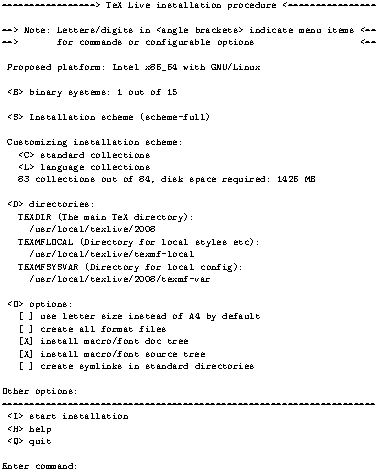
\includegraphics{install08text}}
  \caption{Main menu of the text mode installer}
  \label{fig:text_main_menu}
\end{figure}

\section{\tlu}
\label{sec:texlua}

Nowadays \TeX{} contains a customized copy of Lua as embedded
scripting language. When called as \tlu, it acts as a standalone Lua
interpreter, customized for a \TeX{} environment. This is a very
attractive scripting solution:
\begin{itemize}
\item no version worries: \tlu{} scripts should simply match the
  \TeX{} version they are part of.
\item \tlu{} has \kpse\ compiled in.  In a \tlu{} script \kpse{}
  file searching happens within the same process, which can speed
  things up a lot.
\item An embedded scripting language is immune from the kind of
  bloat suffered by popular scripting languages such as \pl{} and
  Ruby.
\end{itemize}
Under Windows, the |.texlua| extension is made an executable file
type.

\section{Install \tl\ from the Internet}
\label{sec:internet}

It is now possible to install \tl\ from a remote server.  Thanks to
the new infrastructure, the package database which tells the
installer which packages have to be downloaded and how to install
them, is a single file.

Two installers for network downloads are provided.
|install-tl-unx.tar.gz.| supports Unix only.  |install-tl.zip|
additionally contains a small subset of \pl\ for Windows which is
required to bootstrap the system.  The latter works on all platforms
supported by \tl.  The sole reason for providing a separate package
for Unix is its significantly smaller size.


\section{A new compression Algorithm}
\label{sec:lzma}

Using |.tar.lzma| compression instead of |.zip| reduces the size of the
compressed packages by 20\%.  It cannot be assumed that |lzma|
decompressors are available on any platform, hence they have to be
provided for all platforms supported by \tl.  Fortunately there is a
program `|lzmadec|' available for all platforms.  The size of the
executable file is only 12\,kB.

\section{Bringing Windows in line with Unix}

\tl\ 2008 supports Windows 2000 and later. By dropping older Windows
versions, there is much less need to treat Windows specially.

\subsection{\texttt{\$HOME} and multi-user support}
Under Windows 2000 and later, users have a real home directory,
viz. \verb+%USERPROFILE%+, usually
\verb+C:\Documents and Settings\+\textit{username}.

This is now reflected in tilde expansion by \kpse, thanks to Karl
Berry: \verb+~/texmf+ is expanded to \verb+%USERPROFILE%\texmf+
under Windows and to \verb+$HOME/texmf+ under Unix.

It is also possible to differentiate between system settings and
user settings. Now there is no reason any more to have a different
set of \texttt{texmf} trees or to leave out scripts such as
\texttt{fmtutil-sys} and \texttt{updmap-sys}. It also shares the
Unix \texttt{texmf.cnf}.

\subsection{Scripting}
We cannot count on the presence of the usual Unix scripting
languages. We deal with this by including a limited subset of \pl{}
for Windows, which contains just enough modules to run the installer
and the \pl{} scripts which are part of \tl.

To prevent interference with any pre-existing \pl, we make it
invisible to the system by not placing it on the searchpath and by
not creating or changing any \pl-related settings. Instead, the
\tl\ \pl\ scripts are called via wrapper scripts that know how to
find Perl and that create the environment variables it needs for the
duration of the job. In the case of the installer itself, the
wrapper is a simple batchfile (but not so simple that it would have
worked under earlier Windows versions). But in most cases, the
wrapper is written in \tlu; see section \ref{sec:texlua}.

Most likely, there won't be a Bourne-compatible shell either. But in
the new \tl, most shell scripts have been replaced by \pl- and
\tlu{} scripts, which also work under Windows. So we just about got
rid of \texttt{.exe} files replacing Unix scripts.

\subsection{\gs}

\tl{} for Windows also includes a hidden copy of \gs, another
fixture of Unix systems that is usually absent from Windows.  The
most important batch files provided by \gs\ have been ported to
\tlu{}, see \ref{sec:texlua}.

\begin{figure*}[htb]
  \centering
  \resizebox{\textwidth}{!}{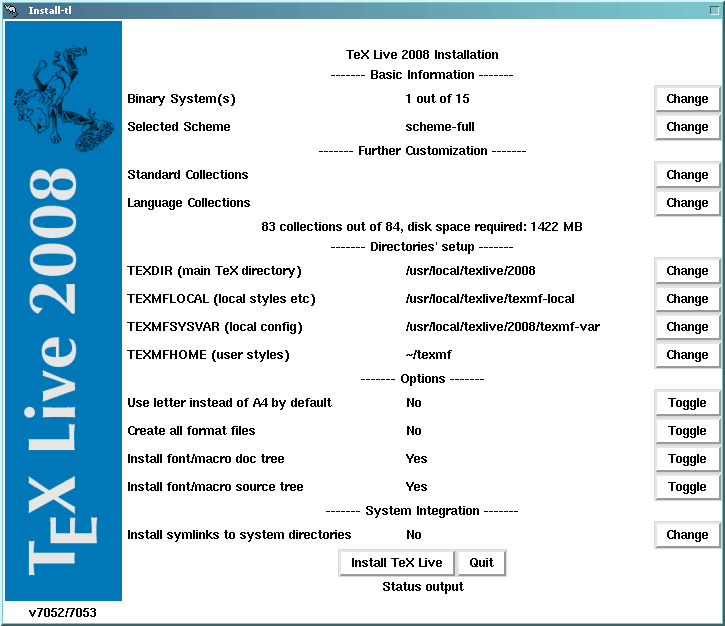
\includegraphics{install08gui}}
  \caption{The main menu of the GUI installer}
  \label{fig:gui_main_menu}
\end{figure*}

\section{Testing with virtual machines}
We do much of our testing with virtual machines. With programs such
as VirtualBox or VMware you can run a guest operating system as a
program inside a host operating system.

Even if host and guest are the same operating system, it is a huge
advantage that the host will be unaffected, and that the guest is
free from the idiosyncrasies of the host.

Normally, the filesystem of the guest is on a virtual disk, which is
a very large file on the host system.  An installation can simply be
reverted by making a fresh copy from backup of this very large file.

The guest can access the \tl{} files via e.g. a shared folder or
Samba, using a virtual network interface. An Internet install can be
simulated with a webserver or ftp server on the host, also via a
virtual network interface. These server programs can simply use the
\tl{} working copy.

\newpage
\begin{thebibliography}{1}
\bibitem{PreiBT08} Norbert \textsc{Preining}
\newblock \emph{The new \TeX~Live Infrastructure and Installer}
Talk held at Bacho\TeX\,2008.
\end{thebibliography}

%\bibliographystyle{arstexnica}
%\bibliography{atsample}

%\end{article}

\end{document}
